\title{VGP-2017-Poster}
%%%%%%%%%%%%%%%%%%%%%%%%%%%%%%%%%%%%%%%%%
% a0poster Portrait Poster
% LaTeX Template
% Version 1.0 (22/06/13)
%
% The a0poster class was created by:
% Gerlinde Kettl and Matthias Weiser (tex@kettl.de)
%
% This template has been downloaded from:
% http://www.LaTeXTemplates.com
%
% License:
% CC BY-NC-SA 3.0 (http://creativecommons.org/licenses/by-nc-sa/3.0/)
%
%%%%%%%%%%%%%%%%%%%%%%%%%%%%%%%%%%%%%%%%%

%-------------------------------------------------------------------------------
%	PACKAGES AND OTHER DOCUMENT CONFIGURATIONS
%-------------------------------------------------------------------------------

\documentclass[a0,portrait]{a0poster}
\usepackage{multicol} % This is so we can have multiple columns of text side-by-side
\columnsep=100pt % This is the amount of white space between the columns in the poster
\columnseprule=3pt % This is the thickness of the black line between the columns in the poster

\usepackage{xcolor}
\usepackage{tcolorbox}

\definecolor{sangertext}{RGB}{7,73,135}
\definecolor{sangersubtitletext}{RGB}{106,185,215}
\definecolor{codepurple}{rgb}{0.58,0,0.82}
\definecolor{backcolour}{rgb}{0.95,0.95,0.92}

% Sanger colour palette
\definecolor{sangerdarkblue}{RGB}{0, 72, 105}
\definecolor{sangermidblue}{RGB}{138, 187, 238}
\definecolor{sangerlightblue1}{RGB}{159, 198, 238}
\definecolor{sangerlightblue2}{RGB}{184, 210, 239}
\definecolor{sangerlightblue3}{RGB}{203, 220, 230}
\definecolor{sangerlightteal}{RGB}{176, 227, 192}
\definecolor{sangerlimegreen}{RGB}{204, 242, 132}
\definecolor{sangerolivegreen}{RGB}{95, 128, 17}
\definecolor{sangerdarkteal}{RGB}{5, 122, 82}
\definecolor{sangermintgreen}{RGB}{221, 246, 164}
\definecolor{sangerdarkbrown}{RGB}{132, 109, 83}
\definecolor{sangerlightbrown}{RGB}{204, 179, 118}
\definecolor{sangerdarkmustard}{RGB}{132, 93, 0}
\definecolor{sangerredbrown}{RGB}{98, 23, 0}
\definecolor{sangerorange}{RGB}{255, 114, 0}
\definecolor{sangerred}{RGB}{195, 0, 29}
\definecolor{sangerdarkred}{RGB}{141, 0, 23}
\definecolor{sangerpurple}{RGB}{124, 0, 79}


\usepackage[scaled=1.0]{helvet}
% \usepackage[scaled=.90]{helvet}

\usepackage{graphicx} % Required for including images
\graphicspath{{figures/}} % Location of the graphics files
\usepackage{booktabs} % Top and bottom rules for table
\usepackage[font=small,labelfont=bf,justification=centering]{caption} % Required for specifying captions to tables and figures
\usepackage{subcaption}
\usepackage{amsfonts, amsmath, amsthm, amssymb} % For math fonts, symbols and environments
\usepackage{wrapfig} % Allows wrapping text around tables and figures
\usepackage{enumerate}
\usepackage[hyphens]{url}
\usepackage{sidecap}
\usepackage[colorlinks,urlcolor=sangerred,linkcolor=black,citecolor=black,linktoc=all]{hyperref}
\setlength{\columnseprule}{0.01pt}
\renewcommand{\columnseprulecolor}{\color[rgb]{0.9,0.9,0.9}}

\renewcommand{\familydefault}{\sfdefault}

\setlength\heavyrulewidth{0.1pt}
\setlength\lightrulewidth{0.1pt}
\setlength{\tabcolsep}{12pt}

\setlength\labelsep   {\dimexpr\labelsep + 0.5em\relax}
\setlength\leftmargini{\dimexpr\leftmargini + 0.5em\relax}

\usepackage{sectsty}
\sectionfont{\color{sangertext}}
\subsectionfont{\color{sangersubtitletext}}

\usepackage[square,numbers]{natbib}

\begin{document}

%-------------------------------------------------------------------------------
%	POSTER HEADER
%-------------------------------------------------------------------------------

\begin{center}
\veryHuge \color{sangertext} \textbf{Plans for scaling vertebrate genome sequencing\\and assembly at the Sanger Institute} \color{sangersubtitletext}
\end{center}

\par\smallskip\noindent
\centerline{\begin{minipage}{0.9\textwidth}
\centering
\Large\color{black}
\textbf{Shane A. McCarthy}\textsuperscript{1},
Marcus Klarqvist\textsuperscript{1},
Milan Malinsky\textsuperscript{1,2},
Dirk-Dominik Dolle\textsuperscript{1},
Hannes Svardal\textsuperscript{1},
Karen Oliver\textsuperscript{1},
Michelle Smith\textsuperscript{1},
Kim Judge\textsuperscript{1},
William Chow\textsuperscript{1},
Mike Quail\textsuperscript{1},
Kerstin Howe\textsuperscript{1},
Thomas Keane\textsuperscript{3},
Richard Durbin\textsuperscript{1}\\
\vspace{0.5cm}
\normalsize
\textsuperscript{1}Wellcome Trust Sanger Institute, Hinxton, Cambridgeshire, CB10 1SA, UK\\
% \hspace{1cm}
\textsuperscript{2}Zoological Institute, Dept. of Environmental Sciences, University of Basel, 4051 Basel, Switzerland\\
\textsuperscript{3}European Bioinformatics Institute, Hinxton, Cambridgeshire, CB10 1SD, UK
\end{minipage}}
\par\smallskip

\vfill

% \hspace{2cm}

\begin{tcolorbox}[boxsep=30pt,width=0.985\textwidth,colback=sangerlightblue3,arc=20pt]
\Large\noindent\color{sangertext}
During 2016-17 the Wellcome Trust Sanger Institute is undertaking a pilot vertebrate genome sequencing project, with the aim to obtain reference quality genome sequences for 50-100 species and additional genome data for a similar number of related species. Our primary focus is on \textbf{fish genomes}, but we are also planning to sequence some \textbf{amphibian} and \textbf{mammalian} species.
\end{tcolorbox}

\vfill

\begin{center}\noindent\rule{1.0\linewidth}{0.05pt}\end{center}

%-------------------------------------------------------------------------------

\begin{multicols}{2}

%-------------------------------------------------------------------------------
%	Project overview
%-------------------------------------------------------------------------------

\section*{Project overview}

During 2016-17 the Wellcome Trust Sanger Institute is undertaking a pilot vertebrate genome sequencing project, with the aim to obtain reference quality genome sequences for 50-100 species and additional genome data for a similar number of related species. Our primary focus is on \textbf{fish genomes}, but we are also planning to sequence some \textbf{amphibian} and \textbf{mammalian} species. Specific targets include:
\vspace{0.5cm}
\begin{tcolorbox}[boxsep=30pt,width=0.48\textwidth,colback=sangerlightteal,arc=20pt]
\large \color{sangertext}
\begin{flushleft}
\begin{itemize}
\setlength{\itemsep}{1.5pt}
\item \textbf{$\sim$30 representatives of fish orders} for which adequate references do not currently exist
\item multiple samples (6 references plus up to 10-20 others) within each of the following fish groups
\begin{itemize}
	\item \textbf{cyprinids} related to the zebrafish \emph{Danio rerio}
	\item \textbf{cichliforms} related to the major haplochromine cichlid evolutionary radiation
	\item \textbf{notothenioid} fish from the Antarctic radiation
	\item \textbf{anabantoid} fish include gouramis
\end{itemize}
\item several \textbf{caecilian} species representing the most basal branch of amphibians
\item \textbf{multiple rodents} with extreme phenotypes providing evolutionary context to mice and rats
\end{itemize}
\end{flushleft}
\end{tcolorbox}
\vspace{0.5cm}
\noindent To collect these samples we are collaborating with multiple members of the Genome10K community and other evolutionary researchers. We are currently using \textbf{Pacific Biosciences Sequel}, \textbf{10X Genomics Chromium} and \textbf{BioNano Irys} as core technologies, and evaluating others including \textbf{Oxford Nanopore} and \textbf{Dovetail}. Our long term aim is to scale up to sequence hundreds then thousands of new species per year.

\vfill
\columnbreak

%-------------------------------------------------------------------------------
%	Project data flow
%-------------------------------------------------------------------------------

\section*{Project data flow}

Data generation and production is being coordinated at the Sanger Insitute, tying in with existing production, R\&D and analysis pipelines. We are collaborating with the European Bioinformatics Institute (EBI) to streamline data deposition into the relevant archives to enable efficient gene annotation and presentation in Ensembl.

\vspace{0.5cm}

\begin{center}
\captionsetup{type=figure}
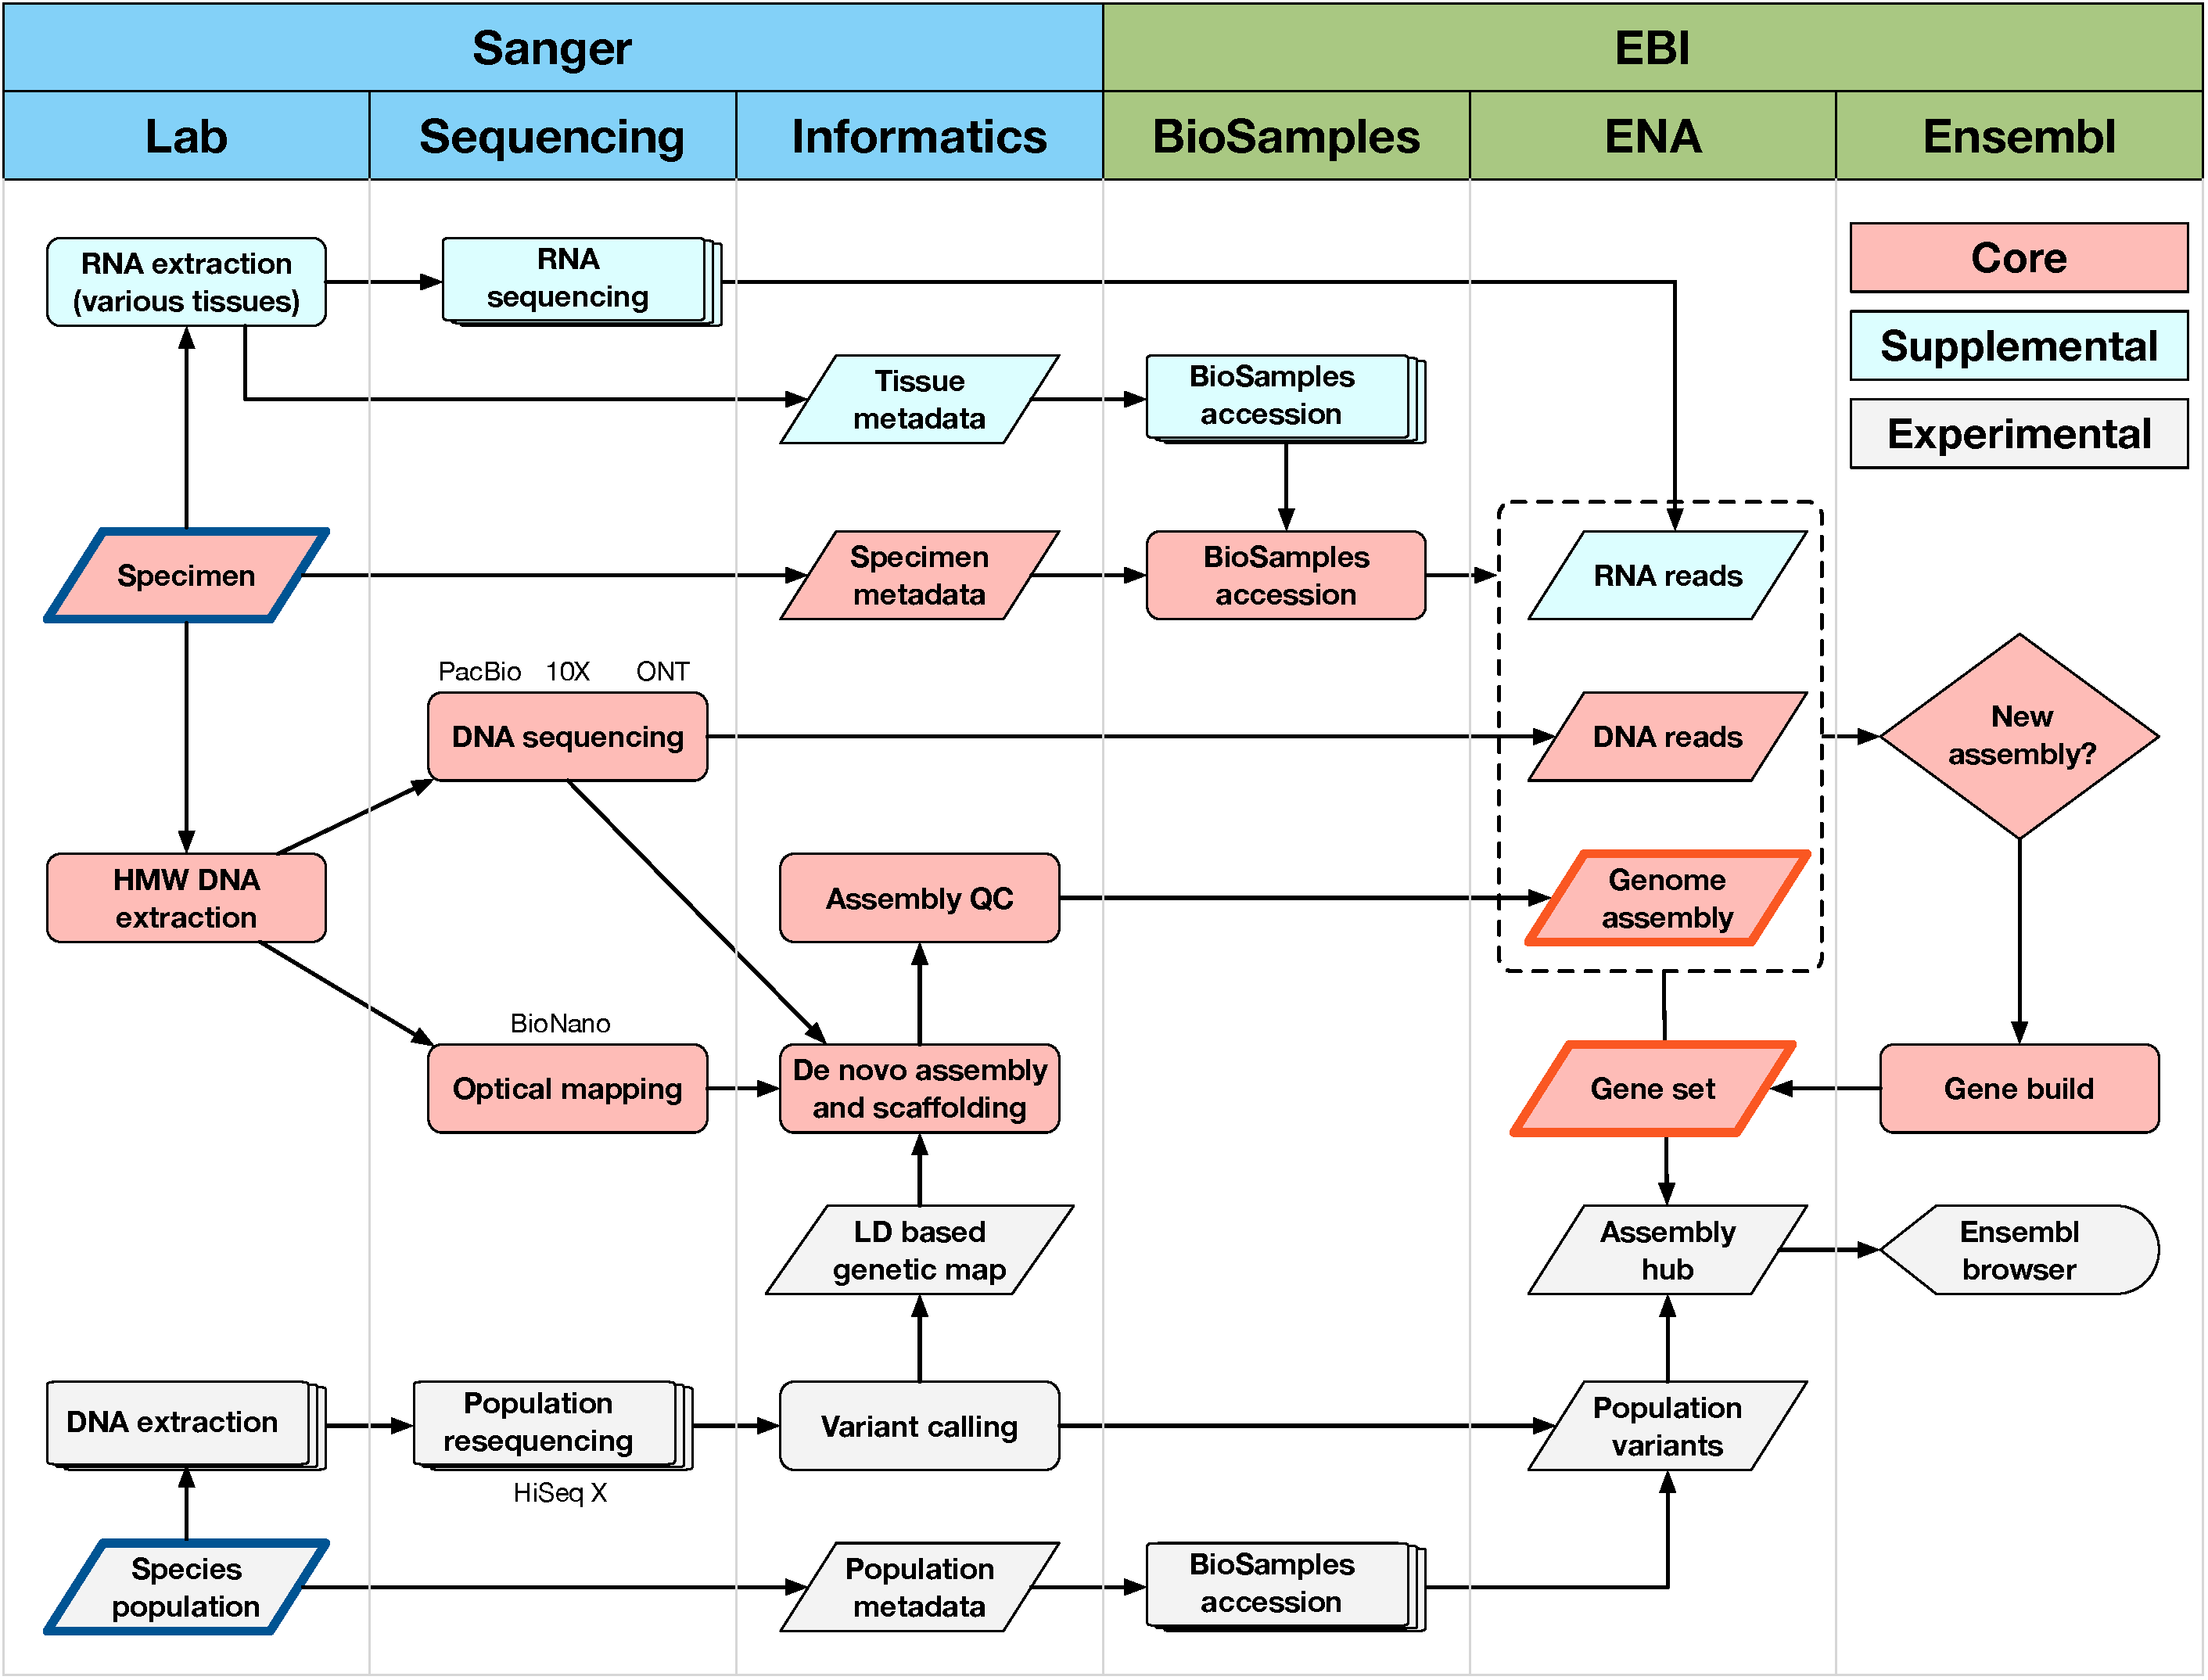
\includegraphics[width=0.9\linewidth]{images/flow.pdf}
\captionof{figure}{Flow diagram for data production for the Vertebrate Genomes Project.}
\end{center}

\end{multicols}

\begin{center}\noindent\rule{1.0\linewidth}{0.05pt}\end{center}

\begin{multicols}{2}

%-------------------------------------------------------------------------------
%	Assembly scaffolding using linkage disequilibrium
%-------------------------------------------------------------------------------

\section*{Assembly scaffolding using linkage disequilibrium}

\emph{Credit: Marcus Klarqvist}

\vspace{0.5cm}

\noindent A key problem in reference genome assembly is to connect together initial contigs or scaffolds, which may have typical size 100kb-10Mb, into chromosome-scale contiguous sequences. As an alternative to physically based methods that use long range restriction maps, read pairs or read sets, we have been investigating using patterns of linkage disequilibrium (LD) between SNPs obtained by low coverage population sequencing. Here we show preliminary results from experiments to reassemble human chromosomes, including a reconstituted map of chromosome 20 and examples of chains of nearby loci in high LD. We are currently exploring applying this approach to scaffold the \emph{Astatotilapia calliptera} assembly.


\begin{center}
\captionsetup{type=figure}
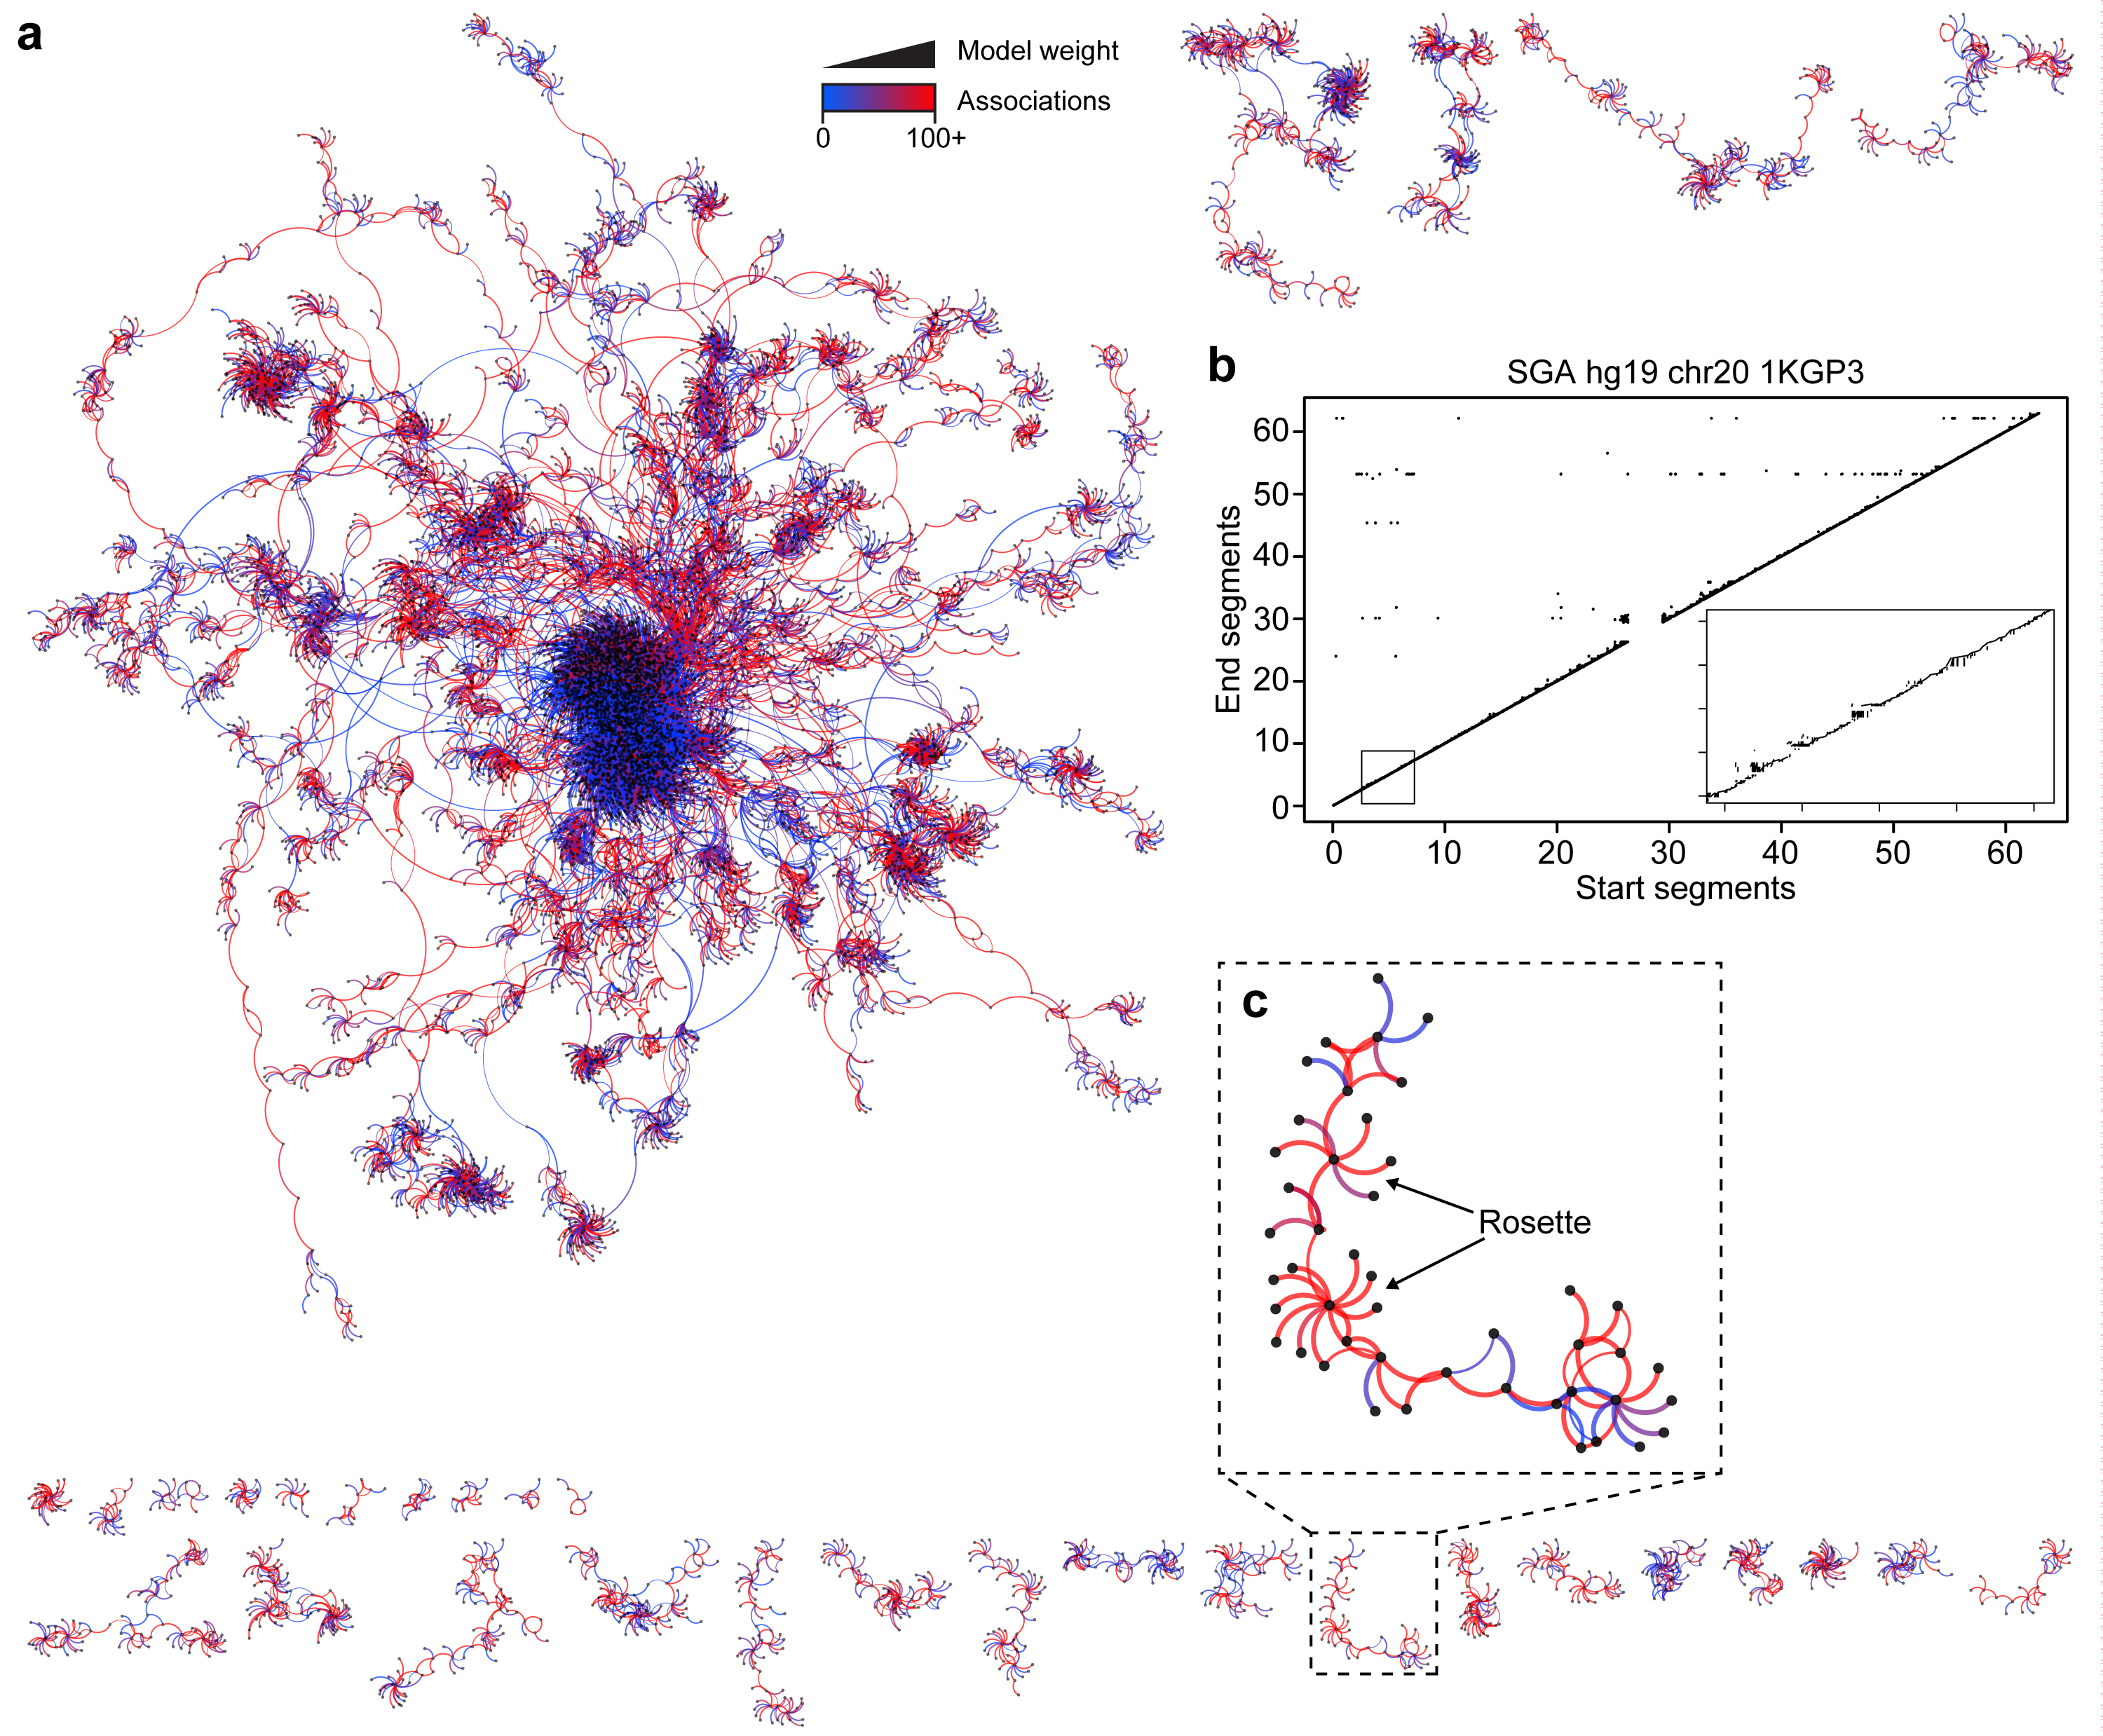
\includegraphics[width=0.9\linewidth]{images/javelin.jpg}
\captionof{figure}{An SGA assembly was made using 30$\times$ Illumina HiSeq X data for NA12878. \textbf{(a)} Graph nodes are the contigs from this SGA assembly with edges indicating an LD association between contigs. The colour of the edges indicates the number of SNPs in association, while the width of the edges indicates the strength of the association. \textbf{(b)} For chromosome 20, we compare the predicted position of the contigs with the truth showing very good agreement. \textbf{(c)} Details of one of the connected components. A rosette is indicative of a number of smaller contigs contained within a larger contig.}
% chr20 - 13,000 contigs (N50 = 10k) all vs all LD is heavy compute.
\end{center}

\vfill

\columnbreak

%-------------------------------------------------------------------------------
%	Preliminary cichlid assemblies
%-------------------------------------------------------------------------------

\section*{Preliminary cichlid assemblies}

\emph{Credit: Milan Malinsky}

\vspace{0.5cm}

\noindent We have recently completed preliminary assemblies for two cichlid species \emph{Astatotilapia calliptera} (fAstCal1, Figure \ref{fAstCal1}) and \emph{Simochromis diagramma} (fSimDia1). We reached a \textbf{contig N50 of 2.47Mb (fAstCal1) and 1.25Mb (fSimDia1)}, with \textbf{assembly sizes of 890Mb and 850Mb} respectively, in agreement with expectations. N50 of fAstCal1 was increased to \textbf{4.2Mb after scaffolding} with BioNano Irys data and \textbf{4.5Mb after scaffolding} with Dovetail Chicago data.
\begin{center}
\captionsetup{type=figure}
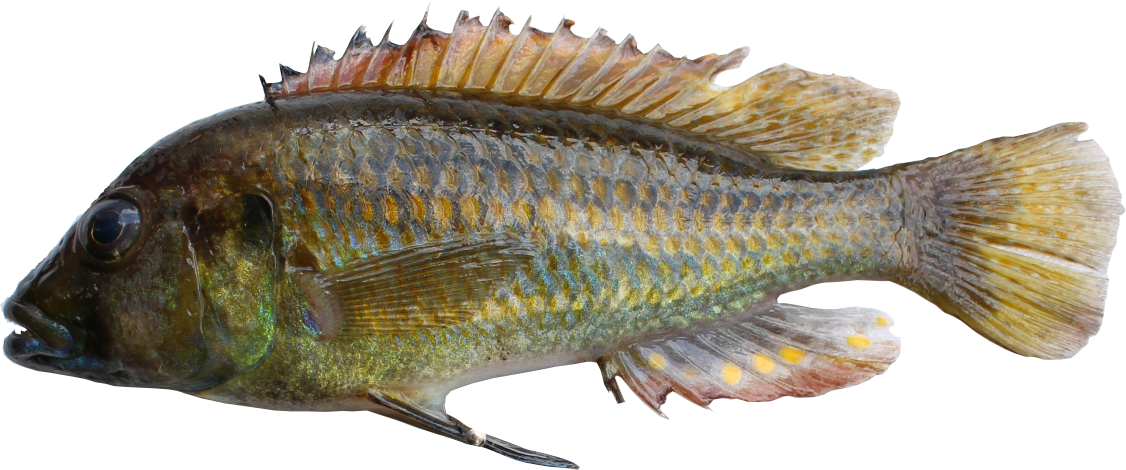
\includegraphics[width=0.7\linewidth]{images/fAstCal1.png}
\captionof{figure}{Eastern happy \emph{Astatotilapia calliptera} from Lake Masoko, Tanzania.}
\label{fAstCal1}
\end{center}

\begin{center}
\captionsetup{type=figure}
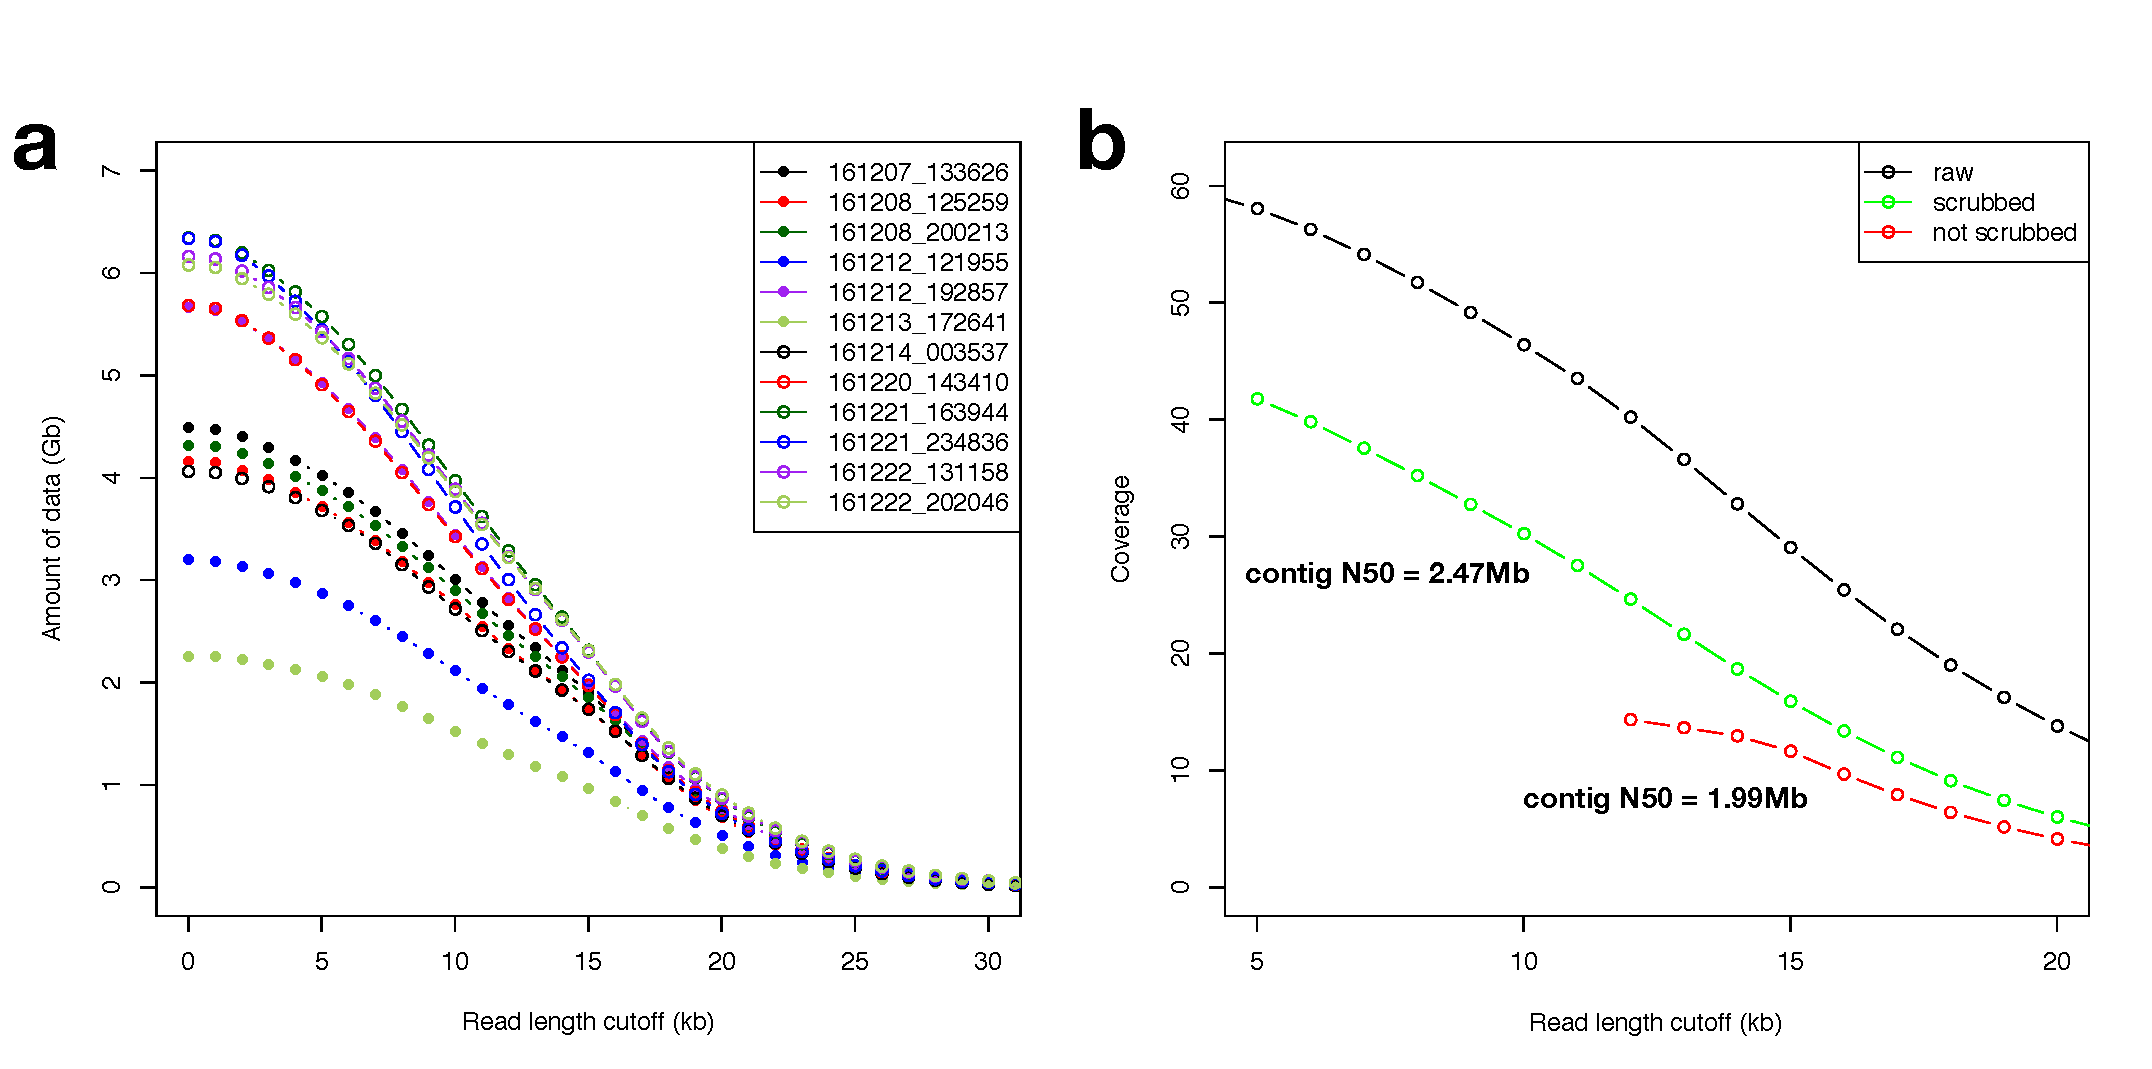
\includegraphics[width=1.0\linewidth]{images/assemblies}
\captionof{figure}{\textbf{(a)} Read length distribution per SMRT cell shows improvement in yield over time. \textbf{(b)} Read scrubbing with Gene Myers' Dazzler pipeline, although it initially removes material and breaks chimeric reads, results in higher coverage after error correction and a resulting improved assembly.}
\end{center}

\vfill

% \begin{tabular}{r|cc}
% % \textbf{sample} & \textbf{fAstCal1} & \textbf{fSimDia1}\\
% \textbf{species} & \emph{Astatotilapia calliptera} & \emph{Simochromis diagramma}\\
% \textbf{technology} & PacBio RSII & PacBio Sequel \\
% \textbf{contig N50} & 2.47~Mb & 1.25~Mb\\
% \textbf{assembly size} & 890~Mb & 850~Mb\\
% \textbf{number of contigs $\ge$ 20kb} & 1100 & 3494\\
% \textbf{scaffold N50 after BioNano} & 4.2~Mb & .\\
% \end{tabular}

\end{multicols}

\vfill

\begin{center}\noindent\rule{1.0\linewidth}{0.05pt}\end{center}

\vfill

\noindent
\begin{minipage}[][][b]{0.4\textwidth}
\begin{tcolorbox}[boxsep=25pt,width=1.0\linewidth,colback=sangerlightblue3,arc=20pt]
\Large{
\color{sangertext}
\textbf{Contact
\hfill
sm15@sanger.ac.uk
\hfill
@mcshane
}}
\end{tcolorbox}
\end{minipage}%
\hfill%
\begin{minipage}[][][b]{0.25\textwidth}
    \centering
    
\includegraphics[height=4cm]{images/wtsi}
\end{minipage}%
\hfill%
\begin{minipage}[][][b]{0.25\textwidth}
    \centering
    
\includegraphics[height=4cm]{images/ebi}
\end{minipage}%

\end{document}